\documentclass{article}
%Para imagenes
\usepackage{graphicx}
\usepackage{wrapfig}
\usepackage{float}
\usepackage{enumitem} % Paquete para personalizar listas
\usepackage[margin=2cm]{geometry} % Ajusta todos los márgenes a 2 centímetros
\usepackage{indentfirst} % Este paquete fuerza la sangría del párrafo en la primera línea
\setlength{\parindent}{1cm} % Ajusta la sangría de los párrafos a 1 cm


\begin{document}
    \begin{titlepage}
        \centering
        {\bfseries\LARGE Universidad de Granada\par}
        \vspace{1cm}
        {\scshape\Large Facultad de Ingeniería Informática \par}
        \vspace{2cm}
        {\scshape\Huge Practica 3: Pruebas software \par}
        \begin{figure}[h]
                \centering
                
\includegraphics[width=0.6\textwidth]{logo_UGR.jpg}
                \label{fig:portada}
            \end{figure}
        {\itshape\Large DS: Grupo 1.7\par}
        \vfill
            {\Large  Emanuel Giraldo Herrera\par}
            {\Large  Thomas Lang \par}
            {\Large  Timur Sorokin \par}
            {\Large  Alejando Iborra Morán \par}
        \vfill
        {\Large (2023-2024) \par}
    \end{titlepage}

\tableofcontents

\newpage
\section{Planificación}

\subsection{"Creador de personajes"}

\begin{itemize}
	\item \textbf{Test 1}: CFG de ClaseBuilder\\
\textbf{Propósito}: Verificar que la función loadCFG() de ClaseBuilder funciona correctamente.

	\item \textbf{Test 2}: CFG de PersonajeBuilder
\\ \textbf{Propósito}: Confirmar que la función loadCFG() de PersonajeBuilder funciona correctamente.


	\item \textbf{Test 3}: Creación correcta del personaje\\
\textbf{Propósito}: Asegurar que la creación de un personaje utilizando PersonajeBuilder se realiza correctamente.


	\item \textbf{Test 4}: Exportación Correcta del personaje
\\\textbf{Propósito}: Verificar que la exportación del personaje se realiza correctamente.


	\item \textbf{Test 5}: Funcionamiento del director
\\ \textbf{Propósito}: Confirmar que el director puede crear un personaje correctamente.


	\item \textbf{Test 6}: Funcionamiento de la fachada
\\ \textbf{Propósito}: Verificar que la fachada funciona como se espera.

\end{itemize}

\subsection{"Gestor de personajes"}
	\begin{itemize}

	\item \textbf{Test 1}: Añadir Personaje
\\ \textbf{Propósito}: Confirmar que se pueden agregar personajes a la lista del gestor.


	\item \textbf{Test 2}: Eliminar Personaje
\\ \textbf{Propósito}: Verificar que se pueden eliminar personajes de la lista del gestor.


	\item \textbf{Test 3}: Ordenar la lista segun el nombre
\\ \textbf{Propósito}: Confirmar que la lista ordenada de la lista segun el nombre funciona correctamente.


    \item \textbf{Test 4}: Ordenar la lista segun la clase
\\ \textbf{Propósito}: Confirmar que la lista ordenada de la lista segun el clase funciona correctamente.


    \item \textbf{Test 5}: Ordernar la lista segun la raza
\\ \textbf{Propósito}: Confirmar que la lista ordenada de la lista segun el raza funciona correctamente.


    \item \textbf{Test 6}: Ordernar la lista segun el atributo
\\ \textbf{Propósito}: Confirmar que la lista ordenada de la lista segun el atributo funciona correctamente.


    \item \textbf{Test 7}: Filtrar la lista segun la clase
\\ \textbf{Propósito}: Confirmar que el filtrado de la lista segun el clase funciona correctamente.


    \item \textbf{Test 8}: Filtrar la lista segun la raza
\\ \textbf{Propósito}: Confirmar que el filtrado de la lista segun el raza funciona correctamente.

\newpage
\section{Análisis}

\subsection{Creador de personajes}

\subsection{CFG de ClaseBuilder}

\textbf{Elemento a Probar}: 

La función loadCFG() de la clase ClaseBuilder.

\textbf{Condiciones para la Prueba}:

        Se requiere que exista un archivo de configuración válido para la clase en cuestión.
        La función loadCFG() debe cargar correctamente los valores del archivo de configuración.
   
\textbf{ Datos Necesarios para la Prueba:}
        Un archivo de configuración válido que contenga los atributos de la clase con sus respectivos valores.
        Valores esperados para cada atributo de la clase según el archivo de configuración.

\subsection{CFG de PersonajeBuilder}

\textbf{Elemento a Probar}:

 La función loadCFG() de la clase PersonajeBuilder.

\textbf{Condiciones para la Prueba}:

        Se requiere que exista un archivo de configuración válido para el personaje en cuestión.
        La función loadCFG() debe cargar correctamente los valores del archivo de configuración.
        
    \textbf{Datos Necesarios para la Prueba:}
    
        Un archivo de configuración válido que contenga los atributos del personaje con sus respectivos valores.
        Valores esperados para cada atributo del personaje según el archivo de configuración.

\subsection{Creación correcta del personaje}

   \textbf{ Elemento a Probar}: 
   
   El proceso de creación de un personaje utilizando PersonajeBuilder.
   
    \textbf{Condiciones para la Prueba:}
        Se deben cargar correctamente los valores de los archivos de configuración de la clase y el personaje.
        Los atributos del personaje creado deben coincidir con los valores esperados según las configuraciones de clase y personaje.
        
    \textbf{Datos Necesarios para la Prueba:}
        Archivos de configuración válidos para la clase y el personaje.
        Valores esperados para los atributos del personaje basados en las configuraciones de clase y personaje.

\subsection{Exportación Correcta del personaje}


    \textbf{Elemento a Probar}:
    
     El proceso de exportación de un personaje.
    
   \textbf{ Condiciones para la Prueba:}
   
        El personaje debe haber sido creado correctamente.
        La función de exportación debe generar un archivo con la estructura correcta y los datos del personaje.
        
    \textbf{Datos Necesarios para la Prueba:}
    
        Un personaje creado y válido.
        Valores esperados para los atributos del personaje en el archivo de exportación.

\subsection{Funcionamiento del director}

   \textbf{ Elemento a Probar:} 
   
   El proceso de creación de un personaje a través del director.
   
   \textbf{ Condiciones para la Prueba:}
        El director debe ser capaz de crear un personaje utilizando un constructor específico.
        
    \textbf{Datos Necesarios para la Prueba:}
    
        Un constructor válido para el tipo de personaje deseado.
        Valores esperados para los atributos del personaje creado.

\subsection{Funcionamiento de la fachada}

   \textbf{ Elemento a Probar:} 
   El funcionamiento de la fachada en una operación específica.
   
    \textbf{Condiciones para la Prueba:}
    
        La fachada debe ser capaz de realizar la operación deseada correctamente.
        
   \textbf{ Datos Necesarios para la Prueba:}
   
        Datos de entrada necesarios para la operación.
        Valores esperados para el resultado de la operación.

\end{itemize}

\subsection{Gestor de personajes}

\subsection{Añadir personajes}

\textbf{Elemento a Probar}: 

La funcion addPersonaje(Personaje) de GestorPersonajes

\textbf{Condiciones para la Prueba}:

        Se requiere que exista un personaje valido ya creado y la instancia de GestorPersonajes
   
\textbf{ Datos Necesarios para la Prueba:}
        Un personaje valido ya creado
        La instancia de GestorPersonajes

\subsection{Eliminar Personajes}

\textbf{Elemento a Probar}:

 La función remPersonaje(indice) de la clase PersonajeBuilder.

\textbf{Condiciones para la Prueba}:

        Se requiere que en GestorPersonajes se haya incluido previamente un personaje valido.
        
    \textbf{Datos Necesarios para la Prueba:}
    
        La instancia de GestorPersonajes con al menos un personaje valido a eliminar.
        El indice de la posicion del personaje a eliminar de GestorPersonajes

\subsection{Ordenar lista de personajes por nombre}

   \textbf{ Elemento a Probar}: 
   
   La funcion ordenarPersonaje(descendente, tipo, atributo) de GestorPersonaje cuando se quiere ordenar la lista por nombre.
   
    \textbf{Condiciones para la Prueba:}
        Se requiere que en GestorPersonajes haya al menos 2 personajes con distinto nombre.

    \textbf{Datos Necesarios para la Prueba:}
        La instancia de GestorPersonajes con al menos 2 personajes de distinto nombre.
        Una variable de opcion para que el orden sea ascendente o descendente.

\subsection{Ordenar lista de personajes por clase}

    \textbf{ Elemento a Probar}: 
    
    La funcion ordenarPersonaje(descendente, tipo, atributo) de GestorPersonaje cuando se quiere ordenar la lista por clase.
    
        \textbf{Condiciones para la Prueba:}
            Se requiere que en GestorPersonajes haya al menos 2 personajes con distinta clase.   
    
        \textbf{Datos Necesarios para la Prueba:}
            La instancia de GestorPersonajes con al menos 2 personajes de distinto clase.
            Una variable de opcion para que el orden sea ascendente o descendente.

\subsection{Ordenar lista de personajes por raza}

    \textbf{ Elemento a Probar}: 
    
    La funcion ordenarPersonaje(descendente, tipo, atributo) de GestorPersonaje cuando se quiere ordenar la lista por raza.
    
        \textbf{Condiciones para la Prueba:}
            Se requiere que en GestorPersonajes haya al menos 2 personajes con distinta raza.    
    
        \textbf{Datos Necesarios para la Prueba:}
            La instancia de GestorPersonajes con al menos 2 personajes de distinto raza.
            Una variable de opcion para que el orden sea ascendente o descendente.

\subsection{Ordenar lista de personajes por atributo}

    \textbf{ Elemento a Probar}: 
    
    La funcion ordenarPersonaje(descendente, tipo, atributo) de GestorPersonaje cuando se quiere ordenar la lista por un atributo.
    
        \textbf{Condiciones para la Prueba:}
            Se requiere que en GestorPersonajes haya al menos 2 personajes con el atributo a ordenar distinto.
    
        \textbf{Datos Necesarios para la Prueba:}
            La instancia de GestorPersonajes con al menos 2 personajes con distinto valor en el atributo a ordenar.
            Una variable de opcion para que el orden sea ascendente o descendente.
            El atributo por el que se quiere ordenar la lista.

\subsection{Filtrar lista de personajes por raza}

    \textbf{ Elemento a Probar}: 
    
    La funcion filtrarPorRaza(raza) de GestorPersonaje cuando se quiere filtrar la lista por una raza especifica.
    
        \textbf{Condiciones para la Prueba:}
            Se requiere que en GestorPersonajes haya al menos un personaje de la raza a filtrar, y al menos un personaje que no pertenezca a esa raza.
    
        \textbf{Datos Necesarios para la Prueba:}
            La instancia de GestorPersonajes con al menos un personaje de la raza a filtrar, y al menos un personaje que no pertenezca a esa raza.

\subsection{Filtrar lista de personajes por clase}

    \textbf{ Elemento a Probar}: 
    
    La funcion filtrarPorClase(clase) de GestorPersonaje cuando se quiere filtrar la lista por una clase especifica.
    
        \textbf{Condiciones para la Prueba:}
            Se requiere que en GestorPersonajes haya al menos un personaje de la clase a filtrar, y al menos un personaje que no pertenezca a esa clase.
    
        \textbf{Datos Necesarios para la Prueba:}
            La instancia de GestorPersonajes con al menos un personaje de la clase a filtrar, y al menos un personaje que no pertenezca a esa clase.


\section{Diseño}
\subsection{Creador de personajes}
\subsubsection{Grupo: Archivos de configuración}
\textbf{TLDR}:
Estos casos de prueba aseguran que los archivos de configuración necesarios para construir personajes estén presentes en el sistema y puedan ser accedidos correctamente por el programa.

\begin{itemize}
	\item \textbf{Casos de prueba}
	\begin{itemize}
		\item Configuración de clase: verificar que los archivos de configuración de clase existen en la ruta especificada
		\item Configuración de raza: verificar que los archivos de configuración de raza existen en la ruta especificada
	\end{itemize}
	\item \textbf{Entorno de prueba}\\
	No se requieren herramientas ni infraestructuras adicionales.

	\item \textbf{Datos de prueba}
	\begin{itemize}
		\item 	Se requiere ClaseBuilder debidamente inicializado.
			\item Se requiere PersonajeBuidler debidamente inicializado.
			\item Se requieren rutas donde se ubican los archivos de configuración.
	\end{itemize}

	
	\item \textbf{Condición base}\\
	Los archivos lib/cfg/* existen y son accesibles. 
\end{itemize}


\subsubsection{Grupo: ClaseBuilder CFG}
\textbf{TLDR:} Verifica que la función \texttt{loadCFG()} de ClaseBuilder carga correctamente los atributos de clase.

\begin{itemize}
	\item \textbf{Casos de prueba:}
	\begin{itemize}
		\item Lectura de atributos de clase: verificar que la función \texttt{loadCFG()} de ClaseBuilder funciona correctamente y carga los atributos de clase esperados.
	\end{itemize}
	
	\item \textbf{Entorno de prueba:}
	\begin{itemize}
		\item No se requieren herramientas ni infraestructuras adicionales.
	\end{itemize}
	
	\item \textbf{Datos de prueba:}
	\begin{itemize}
		\item Se requiere ClaseBuilder debidamente inicializado.
	\end{itemize}
	
	\item \textbf{Condición base:}
	\begin{itemize}
		\item ClaseBuilder está inicializado correctamente y ha cargado los valores desde el archivo de configuración correctamente.
	\end{itemize}
\end{itemize}


\subsubsection{Grupo: PersonajeBuilder CFG}
\textbf{TLDR:} Verifica que la función \texttt{loadCFG()} de PersonajeBuilder carga correctamente los atributos de personaje.

\begin{itemize}
	\item \textbf{Casos de prueba:}
	\begin{itemize}
		\item Lectura de atributos de personaje: verificar que la función \texttt{loadCFG()} de PersonajeBuilder funciona correctamente y carga los atributos de personaje esperados.
	\end{itemize}
	
	\item \textbf{Entorno de prueba:}
	\begin{itemize}
		\item No se requieren herramientas ni infraestructuras adicionales.
	\end{itemize}
	
	\item \textbf{Datos de prueba:}
	\begin{itemize}
		\item Se requiere PersonajeBuilder debidamente inicializado.
	\end{itemize}
	
	\item \textbf{Condición base:}
	\begin{itemize}
		\item PersonajeBuilder está inicializado correctamente  y cha cargado los valores desde el archivo de configuración correctamente.
	\end{itemize}
\end{itemize}


\subsubsection{Grupo: Creación de Personaje}
\textbf{TLDR:} Verifica que la creación de un personaje utilizando los constructores de ClaseBuilder y PersonajeBuilder produce un personaje con los atributos esperados.

\begin{itemize}
	\item \textbf{Casos de prueba:}
	\begin{itemize}
		\item Verificar que los atributos del personaje son los esperados después de su creación.
	\end{itemize}
	
	\item \textbf{Entorno de prueba:}
	\begin{itemize}
		\item No se requieren herramientas ni infraestructuras adicionales.
	\end{itemize}
	
	\item \textbf{Datos de prueba:}
	\begin{itemize}
		\item Se requieren ClaseBuilder y PersonajeBuilder debidamente inicializados.
	\end{itemize}
	
\item \textbf{Condición base:}
\begin{itemize}
	\item ClaseBuilder y PersonajeBuilder están inicializados correctamente y la construcción de los atributos en el builder da el mismo resultado que \texttt{loadCFG()}.
\end{itemize}
\end{itemize}


\subsubsection{Grupo: Exportación del estado}
\textbf{TLDR:} Verifica que la exportación del estado de un personaje se realiza correctamente y que se genera el archivo esperado.

\begin{itemize}
	\item \textbf{Casos de prueba:}
	\begin{itemize}
		\item Verificar que el archivo de exportación del estado del personaje se genera correctamente en la ubicación especificada.
	\end{itemize}
	
	\item \textbf{Entorno de prueba:}
	\begin{itemize}
		\item No se requieren herramientas ni infraestructuras adicionales.
	\end{itemize}
	
	\item \textbf{Datos de prueba:}
	\begin{itemize}
		\item Se requiere un personaje correctamente construido y una ubicación de archivo de exportación válida.
	\end{itemize}
	
	\item \textbf{Condición base:}
	\begin{itemize}
		\item El personaje está correctamente construido y la ubicación de archivo de exportación es válida. Finalmente que el archivo efectivamente se ha creado.
	\end{itemize}
\end{itemize}



\subsubsection{Grupo: Funcionamiento Director}
\textbf{TLDR:} Verifica que el director pueda crear un personaje correctamente y que el personaje creado tenga el nombre esperado.

\begin{itemize}
	\item \textbf{Casos de prueba:}
	\begin{itemize}
		\item Verificar que el director pueda crear un personaje con el nombre especificado.
		\item Verificar que el nombre del personaje creado coincida con el nombre especificado.
	\end{itemize}
	
	\item \textbf{Entorno de prueba:}
	\begin{itemize}
		\item No se requieren herramientas ni infraestructuras adicionales.
	\end{itemize}
	
	\item \textbf{Datos de prueba:}
	\begin{itemize}
		\item Se requiere un director correctamente inicializado y un nombre de personaje válido.
	\end{itemize}
	
	\item \textbf{Condición base:}
	\begin{itemize}
		\item El director está correctamente inicializado y puede crear un personaje con el nombre especificado.
	\end{itemize}
\end{itemize}



\subsubsection{Grupo: Funcionamiento de la Fachada}
\textbf{TLDR:} Verifica que la fachada pueda crear un personaje correctamente con los constructores proporcionados y que el personaje creado tenga el nombre esperado.

\begin{itemize}
	\item \textbf{Casos de prueba:}
	\begin{itemize}
		\item Verificar que la fachada pueda crear un personaje utilizando los constructores de ClaseBuilder y PersonajeBuilder.
		\item Verificar que el nombre del personaje creado coincida con el nombre especificado.
	\end{itemize}
	
	\item \textbf{Entorno de prueba:}
	\begin{itemize}
		\item No se requieren herramientas ni infraestructuras adicionales.
	\end{itemize}
	
	\item \textbf{Datos de prueba:}
	\begin{itemize}
		\item Se requiere una fachada correctamente inicializada, un constructor de ClaseBuilder y PersonajeBuilder válidos, y un nombre de personaje válido.
	\end{itemize}
	
	\item \textbf{Condición base:}
	\begin{itemize}
		\item La fachada está correctamente inicializada y puede crear un personaje utilizando los constructores proporcionados.
	\end{itemize}
\end{itemize}

\subsection{Gestor personajes}
Se encarga de verificar el funcionamiento adecuado del gestor de personajes en el sistema. Este gestor gestiona una la lista de personajes, permitiendo añadir, eliminar y realizar operaciones como ordenar y filtrar por diferentes criterios, como nombre, clase, raza o atributo.

\subsubsection{Añadir Personaje}
\textbf{TLDR:} Este caso de prueba verifica que el gestor de personajes pueda añadir correctamente un personaje a la lista de personajes.

\begin{itemize}
	\item \textbf{Casos de prueba:}
	\begin{itemize}
		\item Se añade un personaje a la lista del gestor de personajes.
	\end{itemize}
	
	\item \textbf{Entorno de prueba:}
	\begin{itemize}
		\item Se necesita un gestor de personajes inicializado y un personaje válido.
	\end{itemize}
	
	\item \textbf{Datos de prueba:}
	\begin{itemize}
		\item Gestor de personajes correctamente inicializado.
		\item Personaje válido.
	\end{itemize}
	
	\item \textbf{Condición base:}
	\begin{itemize}
		\item El gestor de personajes está correctamente inicializado y la lista de personajes está vacía.
	\end{itemize}
	
\end{itemize}

\subsubsection{Eliminar Personaje}
\textbf{TLDR:} Este caso de prueba verifica que el gestor de personajes pueda eliminar correctamente un personaje de la lista de personajes.

\begin{itemize}
	\item \textbf{Casos de prueba:}
	\begin{itemize}
		\item Se elimina un personaje de la lista del gestor de personajes.
	\end{itemize}
	
	\item \textbf{Entorno de prueba:}
	\begin{itemize}
		\item Se necesita un gestor de personajes inicializado y un personaje válido en la lista del gestor.
	\end{itemize}
	
	\item \textbf{Datos de prueba:}
	\begin{itemize}
		\item Gestor de personajes correctamente inicializado.
		\item Personaje válido dentro del gestor.
	\end{itemize}
	
	\item \textbf{Condición base:}
	\begin{itemize}
		\item El gestor de personajes está correctamente inicializado y el personaje esta en la lista del gestor.
	\end{itemize}
	
\end{itemize}

\subsubsection{Ordenar lista por nombre}
\textbf{TLDR:} Este caso de prueba verifica que el gestor de personajes puede ordenar la lista de personajes segun el nombre 

\begin{itemize}
	\item \textbf{Casos de prueba:}
	\begin{itemize}
		\item Se desea ordenar la lista del gestor segun el nombre de los personajes
	\end{itemize}
	
	\item \textbf{Entorno de prueba:}
	\begin{itemize}
		\item Se necesita un gestor de personajes inicializado con varios personajes en su lista y de distinto nombre.
	\end{itemize}
	
	\item \textbf{Datos de prueba:}
	\begin{itemize}
		\item Gestor de personajes correctamente inicializado.
        \item Variable para ordenar la lista de forma ascendente y descendete
		\item Personajes validos dentro de la lista con nombres diferentes
	\end{itemize}
	
	\item \textbf{Condición base:}
	\begin{itemize}
		\item El gestor de personajes está correctamente inicializado y los personajes estan en su lista
	\end{itemize}
	
\end{itemize}

\subsubsection{Ordenar lista por raza}
\textbf{TLDR:} Este caso de prueba verifica que el gestor de personajes puede ordenar la lista de personajes segun el raza 

\begin{itemize}
	\item \textbf{Casos de prueba:}
	\begin{itemize}
		\item Se desea ordenar la lista del gestor segun el raza de los personajes
	\end{itemize}
	
	\item \textbf{Entorno de prueba:}
	\begin{itemize}
		\item Se necesita un gestor de personajes inicializado con varios personajes en su lista y de distinto raza.
	\end{itemize}
	
	\item \textbf{Datos de prueba:}
	\begin{itemize}
		\item Gestor de personajes correctamente inicializado.
        \item Variable para ordenar la lista de forma ascendente y descendete
		\item Personajes validos dentro de la lista con razas diferentes
	\end{itemize}
	
	\item \textbf{Condición base:}
	\begin{itemize}
		\item El gestor de personajes está correctamente inicializado y los personajes estan en su lista
	\end{itemize}
	
\end{itemize}

\subsubsection{Ordenar lista por clase}
\textbf{TLDR:} Este caso de prueba verifica que el gestor de personajes puede ordenar la lista de personajes segun el clase 

\begin{itemize}
	\item \textbf{Casos de prueba:}
	\begin{itemize}
		\item Se desea ordenar la lista del gestor segun el clase de los personajes
	\end{itemize}
	
	\item \textbf{Entorno de prueba:}
	\begin{itemize}
		\item Se necesita un gestor de personajes inicializado con varios personajes en su lista y de distinto clase.
	\end{itemize}
	
	\item \textbf{Datos de prueba:}
	\begin{itemize}
		\item Gestor de personajes correctamente inicializado.
        \item Variable para ordenar la lista de forma ascendente y descendete
		\item Personajes validos dentro de la lista con clase diferentes
	\end{itemize}
	
	\item \textbf{Condición base:}
	\begin{itemize}
		\item El gestor de personajes está correctamente inicializado y los personajes estan en su lista
	\end{itemize}
	
\end{itemize}

\subsubsection{Ordenar lista por atributo}
\textbf{TLDR:} Este caso de prueba verifica que el gestor de personajes puede ordenar la lista de personajes segun el atributo 

\begin{itemize}
	\item \textbf{Casos de prueba:}
	\begin{itemize}
		\item Se desea ordenar la lista del gestor segun el atributo elegido de los personajes
	\end{itemize}
	
	\item \textbf{Entorno de prueba:}
	\begin{itemize}
		\item Se necesita un gestor de personajes inicializado con varios personajes en su lista y que tengan el atributo elegido de distinto valor
	\end{itemize}
	
	\item \textbf{Datos de prueba:}
	\begin{itemize}
		\item Gestor de personajes correctamente inicializado.
        \item Variable para ordenar la lista de forma ascendente y descendete
        \item Atributo a elegir para la lista ordenada
		\item Personajes validos dentro de la lista con con el valor del atributo diferentes
	\end{itemize}
	
	\item \textbf{Condición base:}
	\begin{itemize}
		\item El gestor de personajes está correctamente inicializado y los personajes estan en su lista
	\end{itemize}
	
\end{itemize}

\subsubsection{Filtrar lista por raza}
\textbf{TLDR:} Este caso de prueba verifica que el gestor de personajes puede filtrar la lista de personajes segun la raza 

\begin{itemize}
	\item \textbf{Casos de prueba:}
	\begin{itemize}
		\item Se desea filtrar la lista del gestor segun el raza de los personajes
	\end{itemize}
	
	\item \textbf{Entorno de prueba:}
	\begin{itemize}
		\item Se necesita un gestor de personajes inicializado con varios personajes en su lista, al menos uno de la raza a filtrar y al menos otro de distinta raza.
	\end{itemize}
	
	\item \textbf{Datos de prueba:}
	\begin{itemize}
		\item Gestor de personajes correctamente inicializado.
		\item Personajes validos dentro de la lista, con al menos un personaje de la raza a filtrar y otro de distinta raza.
	\end{itemize}
	
	\item \textbf{Condición base:}
	\begin{itemize}
		\item El gestor de personajes está correctamente inicializado y los personajes estan en su lista.
	\end{itemize}
	
\end{itemize}

\subsubsection{Filtrar lista por clase}
\textbf{TLDR:} Este caso de prueba verifica que el gestor de personajes puede filtrar la lista de personajes segun la clase 

\begin{itemize}
	\item \textbf{Casos de prueba:}
	\begin{itemize}
		\item Se desea filtrar la lista del gestor segun el clase de los personajes
	\end{itemize}
	
	\item \textbf{Entorno de prueba:}
	\begin{itemize}
		\item Se necesita un gestor de personajes inicializado con varios personajes en su lista, al menos uno de la clase a filtrar y al menos otro de distinta raza.
	\end{itemize}
	
	\item \textbf{Datos de prueba:}
	\begin{itemize}
		\item Gestor de personajes correctamente inicializado.
		\item Personajes validos dentro de la lista, con al menos un personaje de la clase a filtrar y otro de distinta clase.
	\end{itemize}
	
	\item \textbf{Condición base:}
	\begin{itemize}
		\item El gestor de personajes está correctamente inicializado y los personajes estan en su lista.
	\end{itemize}
	
\end{itemize}

\newpage
\section{Conclusiones}
\begin{wrapfigure}{l}{0.5\textwidth}
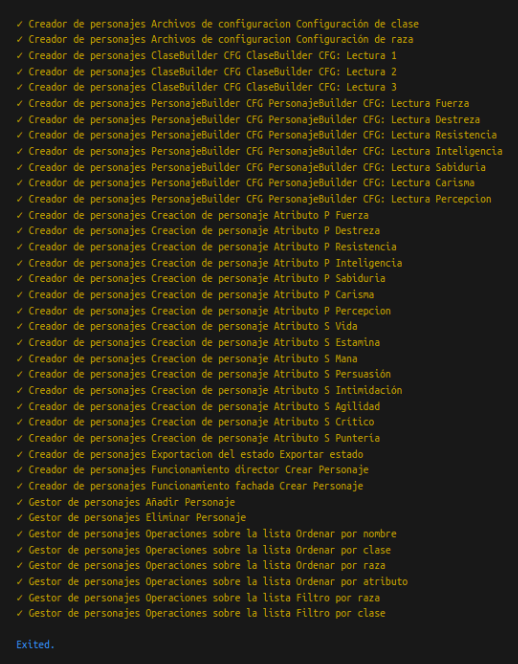
\includegraphics[width=\linewidth]{ejecucion_tests.png}
\end{wrapfigure}
Para realizar las pruebas, hemos integrado dos nuevas funcionalidades en nuestra aplicación:

\begin{itemize}
\item Gestor de personajes: Este componente se encarga de manejar a los personajes en nuestro sistema. Ofrece una interfaz que permite agregar, eliminar y consultar personajes en una lista. Además, ofrece funcionalidades avanzadas como filtrado y ordenamiento sobre el conjunto de personajes.


\item Exportación de estado: Implementamos un método en la clase Personaje para exportar su estado a un archivo de texto. Aunque no especificamos la estructura del archivo en esta etapa, la principal meta era demostrar la capacidad de serializar los datos de un personaje.

\end{itemize}

Cabe mencionar que previamente hemos realizado dos iteraciones sobre este ejercicio. En la primera iteración, durante practica 1, ofreimos una implementación en Java. En la segunda , migramos a Flutter y reescribimos todo el código en Dart. Durante esta migración nos hemos enfrentado con bastantes desafios que finalmente han sido superados. Como resultado de este esfuerzo logramos obtener un código solido y estable que cumple con los requisitos planteados en las practicas anteriores. Debido a esto, durante las pruebas propuestas para esta practica no tuvimos que recurrir a la depuración ni tampoco a realizar cambios en el codigo base. \\


A pesar de no haber surgido problemas durante las pruebas de esta práctica, identificamos algunos puntos que requerían atención y que han sido mitigados a tiempo durante la practica 2 que resumimos a continuación:

\begin{itemize}
\item Builder: Observamos que se reutilizaba la referencia de Personaje en lugar de crear nuevas instancias durante la construcción de personajes. Esto causaba problemas cuando intentábamos guardar varios personajes en una lista, ya que las modificaciones en una referencia afectaban a otras. La solución fue garantizar que cada construcción generara una instancia única del personaje.


\item Archivos de configuración: Detectamos que la ausencia de archivos de configuración causaba fallos en la creación de atributos de personajes. El problema era el uso de caminos absolutos. La solución fue utilizar rutas de archivos relativas. 

\end{itemize}


Aunque el código base demostró ser robusto y confiable, consideramos que la implementación de pruebas y la depuración podrían haber mejorado el proceso de desarrollo. Definir un conjunto claro de requisitos funcionales desde el principio habría agilizado la identificación y resolución de problemas, lo que resultaría en un desarrollo más eficiente y seguro. 





\end{document} 